% Лабораторная работа №1. Метод конечных разностей для ОДУ второго порядка.
\documentclass[12pt,a4paper]{article}

\usepackage[T2A]{fontenc}
\usepackage[utf8]{inputenc}
\usepackage[russian]{babel}

\usepackage{amsmath,amssymb}
\usepackage{graphicx}
\usepackage{booktabs}
\usepackage{array}
\usepackage[left=2.5cm,right=2cm,top=2.5cm,bottom=2.5cm]{geometry}
\usepackage{caption}
\usepackage[hidelinks]{hyperref}

% таблицы: номер и заголовок вверху справа; рисунки: подпись снизу по центру
\captionsetup[table]{position=top,justification=raggedleft,
                     singlelinecheck=false,labelsep=period}
\captionsetup[figure]{position=bottom,justification=centering,
                      singlelinecheck=false,labelsep=period}

\newcommand{\norm}[1]{\left\lVert #1\right\rVert}
\renewcommand{\arraystretch}{1.15}

\newcommand{\Discipline}{Конечно-разностные и сеточные методы}
\newcommand{\WorkKind}{ЛАБОРАТОРНАЯ РАБОТА №\,1}
\newcommand{\WorkTitleA}{Метод конечных разностей для обыкновенного}
\newcommand{\WorkTitleB}{дифференциального уравнения второго порядка}
\newcommand{\StudentGroup}{5030102/30101}
\newcommand{\StudentName}{Никифоров Владислав Дмитриевич}
\newcommand{\TeacherName}{Фролов Максим Евгеньевич}
\newcommand{\TeacherPost}{д.\,ф.-м.\,н., профессор ВШПМиВФ}
\newcommand{\WorkYear}{2026}

\begin{document}

% ---------------------------------------------------------------- титульный лист
\begin{titlepage}
\centering

\vspace*{10mm}

Министерство науки и высшего образования Российской Федерации\\[2mm]
{\large\bfseries Санкт-Петербургский политехнический университет Петра Великого}\\[2mm]
Физико-механический институт\\[1mm]
Высшая школа прикладной математики и вычислительной физики

\vfill

{\Large\bfseries \WorkKind}\\[3mm]
{по дисциплине «\Discipline»}\\[10mm]

{\large \WorkTitleA\\[1.5mm] \WorkTitleB}

\vfill
\vfill

\hspace*{0.2\textwidth}%
\begin{minipage}{0.75\textwidth}
\begin{tabular}{@{}l@{\hspace{4mm}}l@{}}
Выполнил: & студент группы \StudentGroup\\
          & \StudentName\\[5mm]
Проверил: & \TeacherPost\\
          & \TeacherName\\
\end{tabular}
\end{minipage}

\vfill

Санкт-Петербург\\
\WorkYear

\end{titlepage}

\tableofcontents
\newpage

% ---------------------------------------------------------------- 1
\section{Постановка задачи}

\subsection{Общая формулировка}

Рассматривается краевая задача третьего рода для линейного
обыкновенного дифференциального уравнения второго порядка:
\begin{equation}\label{eq:general}
\begin{aligned}
(Au)(x) &:= -\frac{d^2u}{dx^2} + p(x)\frac{du}{dx} + q(x)u = f(x),
   && x\in[a,b],\\[1mm]
(Au)(a) &:= -\alpha_a\frac{du}{dx}(a) + \beta_a u(a) = \gamma_a,
   && \beta_a\ge 0,\\[1mm]
(Au)(b) &:= \alpha_b\frac{du}{dx}(b) + \beta_b u(b) = \gamma_b,
   && \beta_b\ge 0,
\end{aligned}
\end{equation}
где
\[
q(x)\ge c>0,\qquad p(x),\ q(x)\neq \mathrm{const},\qquad
\alpha_a^2+\alpha_b^2\neq 0 .
\]
При этих условиях и $f\in C^2[a,b]$ задача имеет единственное решение
$u\in C^4[a,b]$.

Для того чтобы погрешность численного решения можно было вычислить
точно, задача строится по заранее выбранному решению. Выбирается
функция $u^{\ast}\in C^4[a,b]$ и по ней вычисляются правые части
\[
f^{\ast}(x) := (Au^{\ast})(x),\qquad
\gamma_a^{\ast} := (Au^{\ast})(a),\qquad
\gamma_b^{\ast} := (Au^{\ast})(b).
\]
Решается задача
\begin{equation}\label{eq:test}
(Au)(x) = f^{\ast}(x),\qquad (Au)(a) = \gamma_a^{\ast},\qquad
(Au)(b) = \gamma_b^{\ast},
\end{equation}
единственным решением которой является $u = u^{\ast}$.

\subsection{Выбранные данные}

В работе приняты следующие данные:
\[
[a,b] = [0,3],\qquad p(x) = 1+\sin x,\qquad q(x) = 1+e^{-x},
\]
\[
\alpha_a = 2,\quad \beta_a = 1,\qquad \alpha_b = 1,\quad \beta_b = 0{,}5 .
\]
Коэффициенты непостоянны, $q(x) > 1 = c > 0$, $\beta_a,\beta_b\ge 0$,
так что все условия постановки выполнены.

В качестве точного решения выбрана функция
\[
u^{\ast}(x) = x\cos(x^2),
\]
\[
(u^{\ast})'(x) = \cos(x^2) - 2x^2\sin(x^2),\qquad
(u^{\ast})''(x) = -6x\sin(x^2) - 4x^3\cos(x^2).
\]
Её «частота» растёт с ростом $x$: вблизи левого конца функция меняется
медленно, вблизи правого быстро осциллирует, на отрезке имеется три
экстремума, а амплитуда колебаний растёт (рис.~\ref{fig:exact}).
Вторая производная меняется от нуля при $x=0$ до
$\lvert (u^{\ast})''(3)\rvert\approx 100$, что позволяет хорошо увидеть
особенности разностных схем.

Правые части краевых условий:
\[
\gamma_a^{\ast} = -2\cdot(u^{\ast})'(0) + u^{\ast}(0) = -2,\qquad
\gamma_b^{\ast} = (u^{\ast})'(3) + 0{,}5\,u^{\ast}(3) \approx -9{,}696 .
\]

Для отладки программы использовалась также функция $u^{\ast}(x) = x^2$.

\begin{figure}[htbp]
\centering
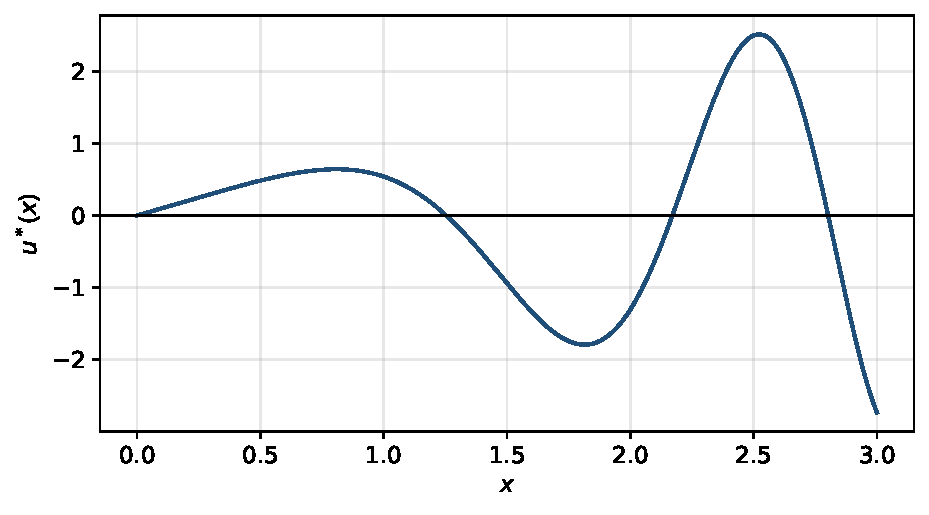
\includegraphics[width=0.85\textwidth]{figures/exact.pdf}
\caption{График точного решения $u^{\ast}(x) = x\cos(x^2)$}
\label{fig:exact}
\end{figure}

% ---------------------------------------------------------------- 2
\section{Разностные схемы}

\subsection{Сетка}

На отрезке $[a,b]$ вводится равномерная сетка
\[
x_i = a + ih,\qquad i = 0,1,\dots,n,\qquad h = \frac{b-a}{n}.
\]
Приближённое решение ищется в виде сеточной функции
$v_h = (y_0,\dots,y_n)$, $y_i\approx u(x_i)$. Обозначим
$p_i = p(x_i)$, $q_i = q(x_i)$, $f_i = f^{\ast}(x_i)$.

\subsection{Внутренние узлы}

Во внутренних узлах $i = 1,\dots,n-1$ производные заменяются
центральными разностями:
\[
u''(x_i) = \frac{u_{i-1}-2u_i+u_{i+1}}{h^2} + O(h^2),\qquad
u'(x_i) = \frac{u_{i+1}-u_{i-1}}{2h} + O(h^2).
\]
Получаем разностное уравнение
\begin{equation}\label{eq:inner}
-\frac{y_{i-1}-2y_i+y_{i+1}}{h^2} + p_i\frac{y_{i+1}-y_{i-1}}{2h}
+ q_i y_i = f_i,
\end{equation}
или, после группировки,
\[
a_i y_{i-1} + b_i y_i + c_i y_{i+1} = f_i,\qquad
a_i = -\frac{1}{h^2}-\frac{p_i}{2h},\quad
b_i = \frac{2}{h^2}+q_i,\quad
c_i = -\frac{1}{h^2}+\frac{p_i}{2h}.
\]
Погрешность аппроксимации уравнения во внутренних узлах равна $O(h^2)$.
Обе рассматриваемые схемы используют~\eqref{eq:inner} и отличаются
только аппроксимацией производной в краевых условиях.

\subsection{Схема $O(h)$}

Производная на концах заменяется односторонней разностью:
\[
u'(a) = \frac{u_1-u_0}{h} + O(h),\qquad
u'(b) = \frac{u_n-u_{n-1}}{h} + O(h).
\]
Краевые условия принимают вид
\[
-\alpha_a\frac{y_1-y_0}{h} + \beta_a y_0 = \gamma_a,\qquad
\alpha_b\frac{y_n-y_{n-1}}{h} + \beta_b y_n = \gamma_b .
\]
Погрешность аппроксимации краевых условий равна $O(h)$, поэтому и вся
схема имеет первый порядок.

\subsection{Схема $O(h^2)$}

По формуле Тейлора
\[
\frac{u_1-u_0}{h} = u'(a) + \frac{h}{2}u''(a) + O(h^2).
\]
Главный член погрешности содержит $u''(a)$, который выражается из
самого уравнения: $u'' = pu' + qu - f$. Подстановка даёт
\[
\frac{u_1-u_0}{h} = u'(a)\left(1+\frac{hp_0}{2}\right)
+ \frac{h}{2}(q_0u_0 - f_0) + O(h^2),
\]
откуда
\[
u'(a) = \frac{\dfrac{u_1-u_0}{h} - \dfrac{h}{2}(q_0u_0-f_0)}
{1+\dfrac{hp_0}{2}} + O(h^2).
\]
Аналогично на правом конце (разность «назад» меняет знаки):
\[
u'(b) = \frac{\dfrac{u_n-u_{n-1}}{h} + \dfrac{h}{2}(q_nu_n-f_n)}
{1-\dfrac{hp_n}{2}} + O(h^2).
\]
Подставив эти выражения в краевые условия и умножив их на
$D_a = 1+hp_0/2$ и $D_b = 1-hp_n/2$ соответственно, получаем
\[
\Bigl(\frac{\alpha_a}{h} + \frac{\alpha_a h q_0}{2} + \beta_a D_a\Bigr)y_0
- \frac{\alpha_a}{h}y_1 = \gamma_a D_a + \frac{\alpha_a h f_0}{2},
\]
\[
-\frac{\alpha_b}{h}y_{n-1}
+ \Bigl(\frac{\alpha_b}{h} + \frac{\alpha_b h q_n}{2} + \beta_b D_b\Bigr)y_n
= \gamma_b D_b + \frac{\alpha_b h f_n}{2}.
\]
Погрешность аппроксимации всей задачи равна $O(h^2)$.

\subsection{Решение системы и проверка программы}

В обеих схемах получается система из $n+1$ линейного уравнения с
трёхдиагональной матрицей. Она решается методом прогонки за $O(n)$
операций. При $h\lvert p_i\rvert/2 < 1$ и $q_i>0$ во внутренних строках
выполнено диагональное преобладание $\lvert b_i\rvert > \lvert a_i\rvert
+ \lvert c_i\rvert$, что обеспечивает устойчивость прогонки.

Программа написана на языке Python (библиотеки NumPy и Matplotlib).
Постановка задачи содержится в файле \texttt{problem.py}, сборка систем
и прогонка~--- в \texttt{schemes.py}, расчёты и построение графиков~---
в \texttt{run.py}.

Для проверки программы решалась задача с $u^{\ast} = x^2$. Так как
$(u^{\ast})''' = (u^{\ast})'''' = 0$, все отброшенные члены в схеме
$O(h^2)$ равны нулю, и она должна воспроизводить это решение точно.
Результаты приведены в табл.~\ref{tab:debug}: погрешность схемы $O(h^2)$
имеет порядок ошибок округления, а погрешность схемы $O(h)$ убывает
пропорционально $h$.

\begin{table}[htbp]
\caption{Погрешность на отладочном решении $u^{\ast} = x^2$}
\label{tab:debug}
\centering
\begin{tabular}{rcc}
\toprule
$n$ & схема $O(h)$ & схема $O(h^2)$\\
\midrule
10 & $2{,}59\cdot10^{-1}$ & $1{,}3\cdot10^{-15}$\\
20 & $1{,}21\cdot10^{-1}$ & $4{,}4\cdot10^{-15}$\\
40 & $5{,}88\cdot10^{-2}$ & $8{,}9\cdot10^{-15}$\\
\bottomrule
\end{tabular}
\end{table}

% ---------------------------------------------------------------- 3
\section{Измерение погрешности}

Погрешность численного решения определяется как
\[
z_h := u_h - v_h,\qquad \norm{z_h} = \max_{0\le i\le n}\lvert u^{\ast}(x_i) - y_i\rvert .
\]
Для сходящейся схемы порядка $k$ имеем $\norm{z_h} = O(h^k)$, и при
малых $h$
\[
\norm{z_h}\approx Ch^k\quad\Longrightarrow\quad
-\lg\norm{z_h}\approx -\lg C + k(-\lg h).
\]
Следовательно, в координатах $(-\lg h,\ -\lg\norm{z_h})$ зависимость
выходит на прямую с угловым коэффициентом $k$. Шаг сетки
последовательно уменьшается в два раза: $n = 20\cdot 2^j$. Эмпирический
порядок оценивается по двум соседним сеткам:
\[
k\approx\log_2\frac{\norm{z_h}}{\norm{z_{h/2}}}.
\]

% ---------------------------------------------------------------- 4
\section{Результаты}

\subsection{Сходимость схем}

На рис.~\ref{fig:compare} показаны численные решения на грубой сетке
$n = 30$. Схема $O(h)$ хорошо приближает решение на левой части
отрезка, где $u^{\ast}$ меняется медленно, но заметно отклоняется вблизи
правого конца. Причина~--- ошибка односторонней разности
$\frac{h}{2}u''(b)$, которая при $\lvert u''(3)\rvert\approx 100$
велика и через краевое условие искажает решение во всей правой части
отрезка. Схема $O(h^2)$ уже при $n=30$ практически совпадает с точным
решением: $\norm{z_h} = 1{,}69$ для схемы $O(h)$ и $0{,}25$ для схемы
$O(h^2)$.

\begin{figure}[htbp]
\centering
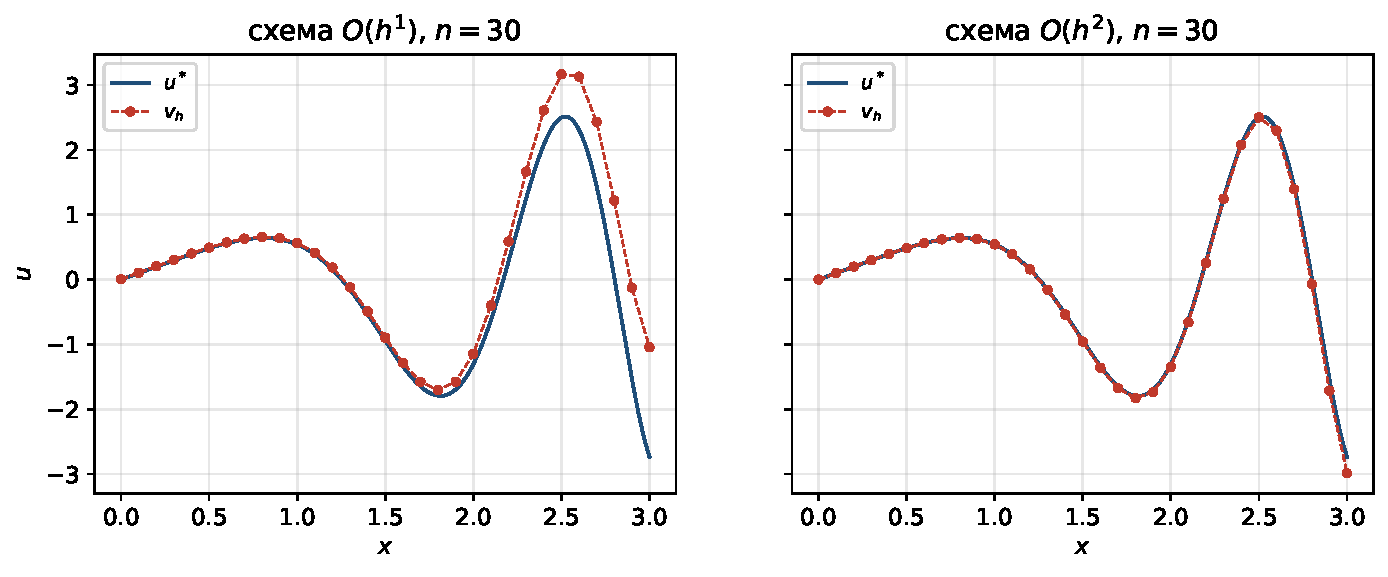
\includegraphics[width=\textwidth]{figures/compare.pdf}
\caption{Точное решение $u^{\ast}$ и численные решения $v_h$ при $n=30$}
\label{fig:compare}
\end{figure}

Погрешности на последовательности сеток приведены в
табл.~\ref{tab:conv} и на рис.~\ref{fig:conv}. Эмпирический порядок
схемы $O(h)$ стремится к единице, схемы $O(h^2)$~--- равен двум уже на
грубых сетках. На графике точки каждой схемы ложатся на прямые,
параллельные эталонным прямым с наклоном $k=1$ и $k=2$. На двух
последних сетках порядок схемы $O(h^2)$ уменьшается до $1{,}98$ и
$1{,}91$: начинают сказываться ошибки округления
(п.~\ref{sec:round}).

\begin{table}[htbp]
\caption{Погрешность схем и эмпирический порядок (двойная точность)}
\label{tab:conv}
\centering
\begin{tabular}{rccccc}
\toprule
$n$ & $h$ & $\norm{z_h}$, $O(h)$ & $k$ & $\norm{z_h}$, $O(h^2)$ & $k$\\
\midrule
20     & $1{,}50\cdot10^{-1}$ & $2{,}430$             & --     & $5{,}752\cdot10^{-1}$ & --\\
40     & $7{,}50\cdot10^{-2}$ & $1{,}294$             & $0{,}91$ & $1{,}425\cdot10^{-1}$ & $2{,}01$\\
80     & $3{,}75\cdot10^{-2}$ & $6{,}660\cdot10^{-1}$ & $0{,}96$ & $3{,}554\cdot10^{-2}$ & $2{,}00$\\
160    & $1{,}88\cdot10^{-2}$ & $3{,}377\cdot10^{-1}$ & $0{,}98$ & $8{,}880\cdot10^{-3}$ & $2{,}00$\\
320    & $9{,}38\cdot10^{-3}$ & $1{,}700\cdot10^{-1}$ & $0{,}99$ & $2{,}220\cdot10^{-3}$ & $2{,}00$\\
640    & $4{,}69\cdot10^{-3}$ & $8{,}528\cdot10^{-2}$ & $1{,}00$ & $5{,}549\cdot10^{-4}$ & $2{,}00$\\
1280   & $2{,}34\cdot10^{-3}$ & $4{,}271\cdot10^{-2}$ & $1{,}00$ & $1{,}387\cdot10^{-4}$ & $2{,}00$\\
2560   & $1{,}17\cdot10^{-3}$ & $2{,}137\cdot10^{-2}$ & $1{,}00$ & $3{,}468\cdot10^{-5}$ & $2{,}00$\\
5120   & $5{,}86\cdot10^{-4}$ & $1{,}069\cdot10^{-2}$ & $1{,}00$ & $8{,}670\cdot10^{-6}$ & $2{,}00$\\
10240  & $2{,}93\cdot10^{-4}$ & $5{,}347\cdot10^{-3}$ & $1{,}00$ & $2{,}168\cdot10^{-6}$ & $2{,}00$\\
20480  & $1{,}46\cdot10^{-4}$ & $2{,}674\cdot10^{-3}$ & $1{,}00$ & $5{,}419\cdot10^{-7}$ & $2{,}00$\\
40960  & $7{,}32\cdot10^{-5}$ & $1{,}337\cdot10^{-3}$ & $1{,}00$ & $1{,}354\cdot10^{-7}$ & $2{,}00$\\
81920  & $3{,}66\cdot10^{-5}$ & $6{,}685\cdot10^{-4}$ & $1{,}00$ & $3{,}432\cdot10^{-8}$ & $1{,}98$\\
163840 & $1{,}83\cdot10^{-5}$ & $3{,}342\cdot10^{-4}$ & $1{,}00$ & $9{,}150\cdot10^{-9}$ & $1{,}91$\\
\bottomrule
\end{tabular}
\end{table}

\begin{figure}[htbp]
\centering
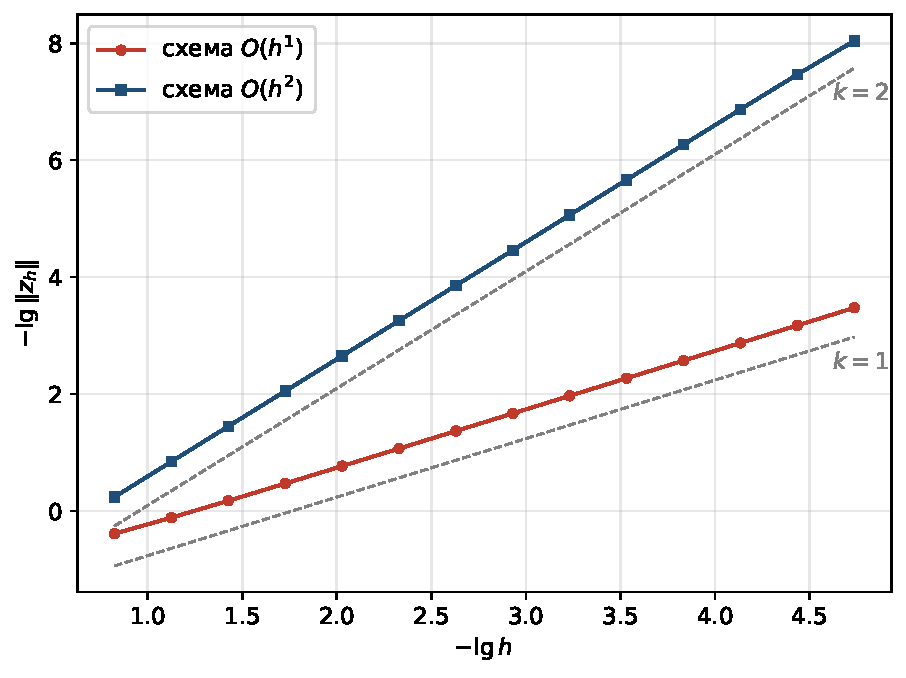
\includegraphics[width=0.75\textwidth]{figures/convergence.pdf}
\caption{Зависимость $-\lg\norm{z_h}$ от $-\lg h$.
Пунктир~--- эталонные прямые с наклоном $k=1$ и $k=2$}
\label{fig:conv}
\end{figure}

\subsection{Влияние ошибок округления}\label{sec:round}

При уменьшении шага погрешность схемы убывает как $h^k$, а погрешность
округления растёт: во второй разности вычитаются близкие числа с
относительной ошибкой $\varepsilon$, а результат делится на $h^2$.
Поэтому полная погрешность ведёт себя как
\[
\norm{z_h}\approx C_1h^k + C_2\frac{\varepsilon}{h^2}
\]
и имеет минимум при некотором шаге. Для чисел одинарной точности
(\texttt{float32}) $\varepsilon\approx 6\cdot10^{-8}$, для двойной
(\texttt{float64}) $\varepsilon\approx 1{,}1\cdot10^{-16}$.

Расчёты были повторены в одинарной точности, а ряд сеток продолжен до
$n\approx1{,}3\cdot10^6$ (табл.~\ref{tab:round}, рис.~\ref{fig:round}).

\begin{table}[htbp]
\caption{Погрешность $\norm{z_h}$ в одинарной и двойной точности}
\label{tab:round}
\centering
\small
\begin{tabular}{rcccc}
\toprule
& \multicolumn{2}{c}{схема $O(h)$} & \multicolumn{2}{c}{схема $O(h^2)$}\\
\cmidrule(lr){2-3}\cmidrule(lr){4-5}
$n$ & double & single & double & single\\
\midrule
20      & $2{,}430$             & $2{,}430$             & $5{,}752\cdot10^{-1}$ & $5{,}752\cdot10^{-1}$\\
40      & $1{,}294$             & $1{,}294$             & $1{,}425\cdot10^{-1}$ & $1{,}425\cdot10^{-1}$\\
80      & $6{,}660\cdot10^{-1}$ & $6{,}660\cdot10^{-1}$ & $3{,}554\cdot10^{-2}$ & $3{,}554\cdot10^{-2}$\\
160     & $3{,}377\cdot10^{-1}$ & $3{,}377\cdot10^{-1}$ & $8{,}880\cdot10^{-3}$ & $8{,}871\cdot10^{-3}$\\
320     & $1{,}700\cdot10^{-1}$ & $1{,}700\cdot10^{-1}$ & $2{,}220\cdot10^{-3}$ & $2{,}215\cdot10^{-3}$\\
640     & $8{,}528\cdot10^{-2}$ & $8{,}536\cdot10^{-2}$ & $5{,}549\cdot10^{-4}$ & $\mathbf{4{,}821\cdot10^{-4}}$\\
1280    & $4{,}271\cdot10^{-2}$ & $4{,}396\cdot10^{-2}$ & $1{,}387\cdot10^{-4}$ & $1{,}245\cdot10^{-3}$\\
2560    & $2{,}137\cdot10^{-2}$ & $\mathbf{1{,}027\cdot10^{-2}}$ & $3{,}468\cdot10^{-5}$ & $2{,}023\cdot10^{-2}$\\
5120    & $1{,}069\cdot10^{-2}$ & $5{,}027\cdot10^{-2}$ & $8{,}670\cdot10^{-6}$ & $5{,}102\cdot10^{-2}$\\
10240   & $5{,}347\cdot10^{-3}$ & $6{,}271\cdot10^{-2}$ & $2{,}168\cdot10^{-6}$ & $6{,}457\cdot10^{-2}$\\
20480   & $2{,}674\cdot10^{-3}$ & $8{,}797\cdot10^{-1}$ & $5{,}419\cdot10^{-7}$ & $8{,}755\cdot10^{-1}$\\
40960   & $1{,}337\cdot10^{-3}$ & $7{,}451\cdot10^{-1}$ & $1{,}354\cdot10^{-7}$ & $7{,}429\cdot10^{-1}$\\
81920   & $6{,}685\cdot10^{-4}$ & $7{,}579\cdot10^{-1}$ & $3{,}432\cdot10^{-8}$ & $7{,}568\cdot10^{-1}$\\
163840  & $3{,}342\cdot10^{-4}$ & $7{,}703\cdot10^{-1}$ & $9{,}150\cdot10^{-9}$ & $7{,}698\cdot10^{-1}$\\
327680  & $1{,}671\cdot10^{-4}$ & $8{,}994\cdot10^{-1}$ & $\mathbf{1{,}474\cdot10^{-9}}$ & $8{,}991\cdot10^{-1}$\\
655360  & $8{,}356\cdot10^{-5}$ & $1{,}156$             & $5{,}953\cdot10^{-9}$ & $1{,}156$\\
1310720 & $4{,}178\cdot10^{-5}$ & $8{,}114\cdot10^{-1}$ & $4{,}066\cdot10^{-9}$ & $8{,}114\cdot10^{-1}$\\
\bottomrule
\end{tabular}

\smallskip
\footnotesize Жирным выделен минимум погрешности в столбце.
\end{table}

\begin{figure}[htbp]
\centering
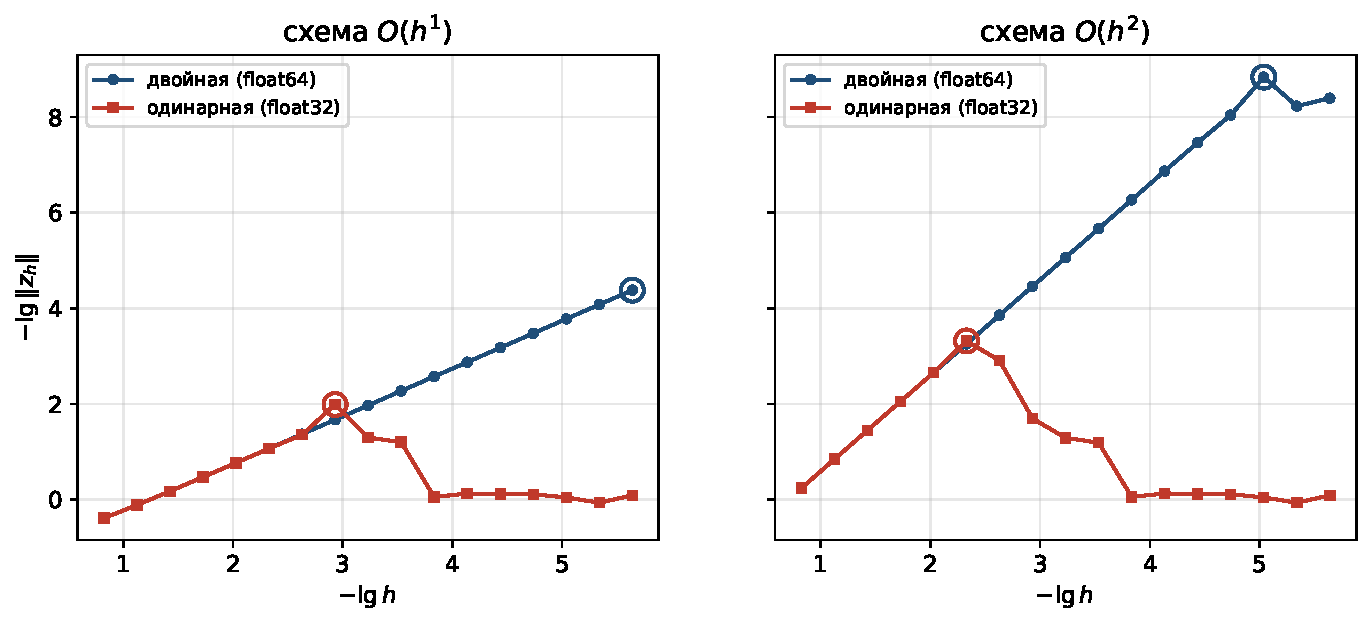
\includegraphics[width=\textwidth]{figures/roundoff.pdf}
\caption{Погрешность в одинарной и двойной точности.
Кружками отмечен минимум погрешности}
\label{fig:round}
\end{figure}

Результаты сведены в табл.~\ref{tab:roundsum}.
\begin{itemize}
\item В одинарной точности для схемы $O(h^2)$ погрешность перестаёт
убывать при $n\approx 640$ ($\norm{z_h}\approx 4{,}8\cdot10^{-4}$); уже
при $n = 1280$ она в 10 раз больше минимальной.
\item Для схемы $O(h)$ в одинарной точности отличие от расчёта в двойной
точности становится заметным при $n\approx 1280$, а рост погрешности
начинается при $n\approx 5000$. Наименьшее значение при $n = 2560$
меньше погрешности самой схемы ($2{,}1\cdot10^{-2}$ в двойной точности),
т.\,е. ошибка округления здесь случайно частично компенсировала ошибку
схемы. При $n\ge 20000$ погрешность обеих схем порядка единицы, и
решение теряет смысл.
\item В двойной точности эффект обнаружен для схемы $O(h^2)$: минимум
$\norm{z_h}\approx 1{,}5\cdot10^{-9}$ при $n = 327\,680$, после чего
погрешность растёт до $(4\text{--}6)\cdot10^{-9}$. Для схемы $O(h)$
собственная погрешность при $n\approx1{,}3\cdot10^6$ ещё порядка
$10^{-5}$, и до уровня ошибок округления она не доходит.
\end{itemize}
Схема $O(h^2)$ раньше упирается в ошибки округления, так как её
собственная погрешность меньше и уравнивается с растущей ошибкой
округления на более грубой сетке.

\begin{table}[htbp]
\caption{Число разбиений, при котором погрешность минимальна}
\label{tab:roundsum}
\centering
\begin{tabular}{lcccc}
\toprule
& \multicolumn{2}{c}{одинарная точность} & \multicolumn{2}{c}{двойная точность}\\
\cmidrule(lr){2-3}\cmidrule(lr){4-5}
Схема & $n$ & $\min\norm{z_h}$ & $n$ & $\min\norm{z_h}$\\
\midrule
$O(h)$   & $\approx 1280$--$2560$ & $\approx 10^{-2}$ & $>1{,}3\cdot10^6$ & $<4{,}2\cdot10^{-5}$\\
$O(h^2)$ & 640 & $4{,}8\cdot10^{-4}$ & 327\,680 & $1{,}5\cdot10^{-9}$\\
\bottomrule
\end{tabular}
\end{table}

\subsection{Число разбиений для заданной точности}

Для каждой точности $\varepsilon_0$ найдено наименьшее $n$, при котором
$\norm{z_h}\le\varepsilon_0$ (двойная точность). Поиск выполнялся так:
$n$ удваивалось до достижения точности, затем уточнялось двоичным
поиском. Результаты приведены в табл.~\ref{tab:nodes}.

\begin{table}[htbp]
\caption{Наименьшее число разбиений $n$, обеспечивающее
$\norm{z_h}\le\varepsilon_0$}
\label{tab:nodes}
\centering
\begin{tabular}{ccccc}
\toprule
& \multicolumn{2}{c}{схема $O(h)$} & \multicolumn{2}{c}{схема $O(h^2)$}\\
\cmidrule(lr){2-3}\cmidrule(lr){4-5}
$\varepsilon_0$ & $n$ & $\norm{z_h}$ & $n$ & $\norm{z_h}$\\
\midrule
$10^{-1}$ & 546      & $9{,}990\cdot10^{-2}$ & 48     & $9{,}886\cdot10^{-2}$\\
$10^{-2}$ & 5\,475   & $9{,}999\cdot10^{-3}$ & 151    & $9{,}970\cdot10^{-3}$\\
$10^{-3}$ & 54\,762  & $1{,}000\cdot10^{-3}$ & 477    & $9{,}990\cdot10^{-4}$\\
$10^{-4}$ & 547\,630 & $1{,}000\cdot10^{-4}$ & 1\,508 & $9{,}995\cdot10^{-5}$\\
$10^{-5}$ & $>2\cdot10^6$ & --              & 4\,768 & $9{,}998\cdot10^{-6}$\\
$10^{-6}$ & $>2\cdot10^6$ & --              & 15\,077 & $9{,}999\cdot10^{-7}$\\
$10^{-7}$ & $>2\cdot10^6$ & --              & 47\,664 & $9{,}987\cdot10^{-8}$\\
\bottomrule
\end{tabular}
\end{table}

Для уменьшения погрешности в 10 раз схеме $O(h)$ требуется в 10 раз
больше разбиений, а схеме $O(h^2)$~--- в $\sqrt{10}\approx3{,}16$ раза
больше, что соответствует порядкам схем. Для точности $10^{-5}$ схеме
$O(h)$ потребовалось бы около $5{,}5\cdot10^6$ разбиений, а схеме
$O(h^2)$ достаточно $4768$.

\subsection{Оценка погрешности по методу Рунге}

Пусть $v_h$ и $v_{h/2}$~--- решения на сетках с шагом $h$ и $h/2$, а
схема имеет порядок $k$. Тогда
$u - v_h\approx Ch^k$, $u - v_{h/2}\approx C(h/2)^k$, и в общих узлах
обеих сеток
\[
u - v_{h/2}\approx R := \frac{v_{h/2} - v_h}{2^k-1}.
\]
Величина $R$ даёт оценку погрешности без использования точного решения.
Уточнённое решение строится как
\[
v_{\text{уточн}} = v_{h/2} + R .
\]

Результаты приведены в табл.~\ref{tab:runge1}, \ref{tab:runge2} и на
рис.~\ref{fig:runge}. Отношение оценки к истинной погрешности
$\norm{R}/\norm{z_{h/2}}$ стремится к единице: для схемы $O(h)$ оно
равно $0{,}88$ при $n=20$ и $0{,}997$ при $n=640$, для схемы $O(h^2)$
уже при $n=20$ равно $1{,}01$. Таким образом, метод Рунге даёт
надёжную оценку погрешности.

\begin{table}[htbp]
\caption{Метод Рунге для схемы $O(h)$}
\label{tab:runge1}
\centering
\begin{tabular}{rccccc}
\toprule
$n$ & $\norm{R}$ & $\norm{z_{h/2}}$ & $\norm{R}/\norm{z_{h/2}}$ &
$\norm{u - v_{\text{уточн}}}$ & порядок\\
\midrule
20    & $1{,}135$             & $1{,}294$             & $0{,}877$ & $1{,}589\cdot10^{-1}$ & --\\
40    & $6{,}282\cdot10^{-1}$ & $6{,}660\cdot10^{-1}$ & $0{,}943$ & $3{,}780\cdot10^{-2}$ & $2{,}07$\\
80    & $3{,}284\cdot10^{-1}$ & $3{,}377\cdot10^{-1}$ & $0{,}972$ & $9{,}295\cdot10^{-3}$ & $2{,}02$\\
160   & $1{,}677\cdot10^{-1}$ & $1{,}700\cdot10^{-1}$ & $0{,}986$ & $2{,}309\cdot10^{-3}$ & $2{,}01$\\
320   & $8{,}470\cdot10^{-2}$ & $8{,}528\cdot10^{-2}$ & $0{,}993$ & $5{,}759\cdot10^{-4}$ & $2{,}00$\\
640   & $4{,}257\cdot10^{-2}$ & $4{,}271\cdot10^{-2}$ & $0{,}997$ & $1{,}438\cdot10^{-4}$ & $2{,}00$\\
1280  & $2{,}134\cdot10^{-2}$ & $2{,}137\cdot10^{-2}$ & $0{,}998$ & $3{,}593\cdot10^{-5}$ & $2{,}00$\\
2560  & $1{,}068\cdot10^{-2}$ & $1{,}069\cdot10^{-2}$ & $0{,}999$ & $8{,}981\cdot10^{-6}$ & $2{,}00$\\
5120  & $5{,}345\cdot10^{-3}$ & $5{,}347\cdot10^{-3}$ & $1{,}000$ & $2{,}245\cdot10^{-6}$ & $2{,}00$\\
10240 & $2{,}673\cdot10^{-3}$ & $2{,}674\cdot10^{-3}$ & $1{,}000$ & $5{,}612\cdot10^{-7}$ & $2{,}00$\\
20480 & $1{,}337\cdot10^{-3}$ & $1{,}337\cdot10^{-3}$ & $1{,}000$ & $1{,}405\cdot10^{-7}$ & $2{,}00$\\
\bottomrule
\end{tabular}
\end{table}

\begin{table}[htbp]
\caption{Метод Рунге для схемы $O(h^2)$}
\label{tab:runge2}
\centering
\begin{tabular}{rccccc}
\toprule
$n$ & $\norm{R}$ & $\norm{z_{h/2}}$ & $\norm{R}/\norm{z_{h/2}}$ &
$\norm{u - v_{\text{уточн}}}$ & порядок\\
\midrule
20   & $1{,}442\cdot10^{-1}$ & $1{,}425\cdot10^{-1}$ & $1{,}012$ & $1{,}756\cdot10^{-3}$  & --\\
40   & $3{,}565\cdot10^{-2}$ & $3{,}554\cdot10^{-2}$ & $1{,}003$ & $1{,}077\cdot10^{-4}$  & $4{,}03$\\
80   & $8{,}887\cdot10^{-3}$ & $8{,}880\cdot10^{-3}$ & $1{,}001$ & $6{,}697\cdot10^{-6}$  & $4{,}01$\\
160  & $2{,}220\cdot10^{-3}$ & $2{,}220\cdot10^{-3}$ & $1{,}000$ & $4{,}181\cdot10^{-7}$  & $4{,}00$\\
320  & $5{,}549\cdot10^{-4}$ & $5{,}549\cdot10^{-4}$ & $1{,}000$ & $2{,}612\cdot10^{-8}$  & $4{,}00$\\
640  & $1{,}387\cdot10^{-4}$ & $1{,}387\cdot10^{-4}$ & $1{,}000$ & $1{,}633\cdot10^{-9}$  & $4{,}00$\\
1280 & $3{,}468\cdot10^{-5}$ & $3{,}468\cdot10^{-5}$ & $1{,}000$ & $1{,}000\cdot10^{-10}$ & $4{,}03$\\
2560 & $8{,}670\cdot10^{-6}$ & $8{,}670\cdot10^{-6}$ & $1{,}000$ & $6{,}267\cdot10^{-12}$ & $4{,}00$\\
5120 & $2{,}168\cdot10^{-6}$ & $2{,}168\cdot10^{-6}$ & $1{,}000$ & $2{,}519\cdot10^{-11}$ & --\\
\bottomrule
\end{tabular}

\smallskip
\footnotesize В последней строке погрешность уточнённого решения
определяется ошибками округления.
\end{table}

\begin{figure}[htbp]
\centering
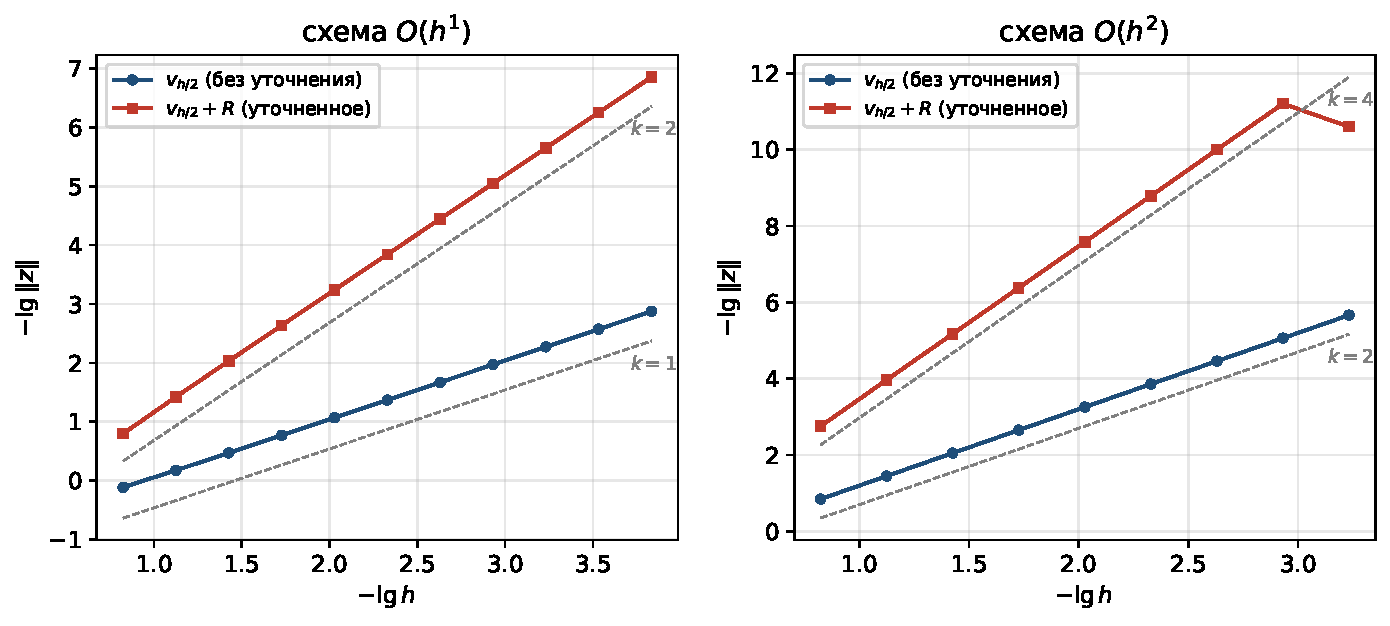
\includegraphics[width=\textwidth]{figures/runge.pdf}
\caption{Погрешность решения $v_{h/2}$ до и после уточнения по Рунге.
Пунктир~--- эталонные прямые}
\label{fig:runge}
\end{figure}

Уточнение повышает порядок точности:
\begin{itemize}
\item для схемы $O(h)$ уточнённое решение имеет порядок $2$;
\item для схемы $O(h^2)$ уточнённое решение имеет порядок $4$.
\end{itemize}
Уточнение по Рунге исключает главный член разложения погрешности, и
порядок уточнённого решения определяется следующим членом. Погрешность
схемы $O(h)$ раскладывается по всем степеням $h$, поэтому после
исключения члена $Ch$ остаётся член порядка $h^2$. Для схемы $O(h^2)$
полученный порядок $4$ означает, что член $h^3$ в разложении
погрешности отсутствует: центральные разности во внутренних узлах
содержат в разложении только чётные степени $h$, а краевые условия
аппроксимированы с использованием самого уравнения. На паре сеток $n=640$ и $1280$
уточнённое решение имеет погрешность $1{,}6\cdot10^{-9}$, тогда как
схеме $O(h^2)$ без уточнения для этого понадобилось бы более
$3\cdot10^5$ разбиений. При $n = 5120$ погрешность уточнённого решения
достигает уровня ошибок округления ($\sim10^{-11}$) и далее не убывает.

% ---------------------------------------------------------------- 5
\section{Выводы}

\begin{enumerate}
\item Построены и реализованы две разностные схемы для краевой задачи
третьего рода. Во внутренних узлах обе используют центральные
разности; краевые условия аппроксимированы односторонней разностью
(схема $O(h)$) либо с уточнением по формуле Тейлора и подстановкой
уравнения (схема $O(h^2)$). Системы решаются методом прогонки.
Корректность программы подтверждена на решении $u^{\ast}=x^2$, которое
схема $O(h^2)$ воспроизводит с машинной точностью.

\item Численно подтверждены теоретические порядки сходимости:
эмпирический порядок равен $1{,}00$ и $2{,}00$ соответственно. Порядок
всей схемы определяется худшей из аппроксимаций: ошибка $O(h)$ в
краевом условии понижает порядок схемы, несмотря на аппроксимацию
$O(h^2)$ во внутренних узлах. На выбранном решении это проявляется
особенно сильно у правого конца, где велика $u''$.

\item Ошибки округления ограничивают достижимую точность. В одинарной
точности погрешность перестаёт убывать уже при $n\approx640$ для схемы
$O(h^2)$ (минимум $4{,}8\cdot10^{-4}$) и при $n\approx1000$--$2500$ для
схемы $O(h)$ (минимум $\approx10^{-2}$); при $n\ge 20000$ решение теряет
смысл. В двойной точности эффект наблюдается для схемы $O(h^2)$ при
$n\approx3\cdot10^5$ (минимум $1{,}5\cdot10^{-9}$).

\item Схема $O(h^2)$ значительно экономичнее: для точности $10^{-4}$ ей
нужно $1508$ разбиений против $547\,630$ у схемы $O(h)$, а точность
$10^{-5}$ и выше схемой $O(h)$ на сетках до $2\cdot10^6$ узлов не
достигается.

\item Метод Рунге даёт надёжную апостериорную оценку погрешности: её
отношение к истинной погрешности близко к единице. Уточнённое по Рунге
решение имеет порядок $2$ для схемы $O(h)$ и порядок $4$ для схемы
$O(h^2)$, что позволяет получать погрешность порядка $10^{-9}$ на сетках
из нескольких сотен узлов.
\end{enumerate}

\end{document}
